\chapter{پیش‌بینی عملکرد پروتئین‌ها با استفاده از گرافلت کرنل گاوسی}\label{chap:protein_function_prediction}

پروتئین‌ها بخش مهمی از فعالیت‌های زیستی را تشکیل می‌دهند. درک نحوه کار آن‌ها وابسته به یافتن عملکرد و وظیفه هر کدام در سامانه‌های زیستی است. مطالعه پروتئین‌ها و پیش‌بینی ساختار و عملکرد آن‌ها، بخش مهمی از بیوانفورماتیک به نام \خمیده{بیوانفورماتیک ساختاری}\پانوشت{\متن‌لاتین{Structural bioinformatics}} را تشکیل می‌دهد. در این فصل از پایان‌نامه، بعد از مرور مفاهیم مورد نیاز، نگاهی به روش‌های پیش‌بینی عملکرد پروتئین بر مبنای SVM خواهیم داشت و گرافلت کرنل گاوسی را با این روش‌ها مقایسه خواهیم کرد.

\section{پروتئین‌ها}\label{sec:protein-structure}
پروتئین‌ها مواد آلی بزرگ و یکی از انواع درشت مولکول‌های زیستی هستند که از \خمیده{اسیدهای آمینه} ساخته شده‌اند. هر اسیدآمینه، از یک کربن نامتقارن به نام کربن آلفا تشکیل یافته است که با چهار گروه مختلف کربوکسیل (\متن‌لاتین{COOH})، اتم هیدروژن، گروه آمینه (\متن‌لاتین{NH2}) و یک زنجیره جانبی (R) ارتباط برقرار می‌کند (شکل \ارجا{fig:aminoacid}). تغییر در زنجیره جانبی، نوع متفاوتی از اسیدآمینه را بوجود می‌آورد که مبنای نامگذاری آن‌هاست. حدود پانصد اسیدآمینه تاکنون شناسایی شده‌است\جستار{Wagner_1983} که ۲۰ عدد از آن‌ها در ساختمان پروتئین‌ها مشارکت دارند. در بین این ۲۰ اسیدآمینه، به غیر از گلیسین\پانوشت{Glycine} که زنجیره جانبی آن یک اتم هیدروژن است، مابقی در زنجیره جانبی خود چند اتم کربن دارند که آن‌ها را به ترتیب فاصله از اتم کربن آلفا با حروف یونانی بتا، گاما و دلتا نامگذاری می‌کنند.

\begin{figure}[h]
\center{
\begin{tikzpicture}[scale=1.5,transform shape,node distance=0.8cm,minimum size=0.40cm,inner sep=0,font=\tiny,
h/.style={circle,draw,thick,align=center,minimum size=0.30cm},
c/.style={circle,draw,thick,align=center,minimum size=0.40cm},
o/.style={circle,draw,thick,align=center,minimum size=0.60cm},
n/.style={circle,draw,thick,align=center,minimum size=0.50cm},
R/.style={rectangle,draw,thick,align=center,minimum size=0.80cm}]
% 2-node
    \node[h] (1) {H};
    \node[h] (2) [below of=1] {H};
    \node[n] (3) [below right=0.14cm and 0.25cm of 1] {N};
    \node[c] (4) [right of=3] {C};
    \node[h] (5) [below=-0.9cm of 4] {H};
    \node[R] (10) [below=0.4cm of 4] {R};
    \node[c] (6) [right of=4] {C};
    \node[o] (7) [below right=-0.9cm and 0.25cm of 6] {O};
    \node[o] (8) [below right=0.2cm and 0.25cm of 6] {O};
    \node[h] (9) [below=-1.1cm of 7] {H};
    \path (1) edge (3);
    \path (2) edge (3);
    \path (3) edge (4);
    \path (4) edge (5);
    \path (4) edge (6);
    \path (4) edge (10);
    \path (7) edge (6);
    \path (8) edge (6);
    \path (7) edge (9);
\end{tikzpicture}
}
\caption{
ساختار اسید‌های آمینه. هر اسیدآمینه از یک کربن آلفا تشکیل شده که با یک گروه آمینه(\متن‌لاتین{NH2})، یک گروه کربوکسیل (\متن‌لاتین{COOH}) و یک زنجیره جانبی (\متن‌لاتین{R}) ارتباط دارد.
}
\label{fig:aminoacid}
\end{figure}

با پیوند اسیدهای آمینه به صورت زنجیره‌‌ای بلند در فرآیند تولید پروتئین توسط سلول، یک \خمیده{پلی‌پپتید} بوجود می‌آید که در اصطلاح، \خمیده{ساختار اول} پروتئین را تشکیل می‌دهد. یعنی در ساده‌ترین حالت، پروتئین یک رشته طولانی ۲۰ حرفی از اسیدهای آمینه است. با برقراری پیوندهای هیدروژنی بین گروه آمینی و گروه کربوکسیل اسیدهای آمینه، نظم‌های موضعی در پروتئین به وجود می‌آید که به آن‌ \خمیده{ساختار دوم} پروتئین گفته می‌شود. \خمیده{مارپیچ آلفا}\پانوشت{\متن‌لاتین{alpha helix}} و \خمیده{صفحه بتا}\پانوشت{\متن‌لاتین{beta sheet}} دو نوع اصلی ساختار دوم هستند. با ورود زنجیره به فضای سلول و طی فرآیند تاشدگی\پانوشت{folding}، پروتئین شکل سه بعدی تقریباً ثابتی به خود می‌گیرد که به آن \خمیده{ساختار سوم} پروتئین گفته می‌شود. بعضی پروتئین‌ها از بیش از یک زنجیره پلی‌پتیدی بوجود می‌آیند. به نحوه قرار گرفتن این زنجیره‌ها در فضای سه‌بعدی، \خمیده{ساختار چهارم} پروتئین می‌گویند. شکل \ارجا{fig:protein} این مفاهیم را در قالب تصویر نشان می‌دهد.

\begin{figure}[h!]
\center{
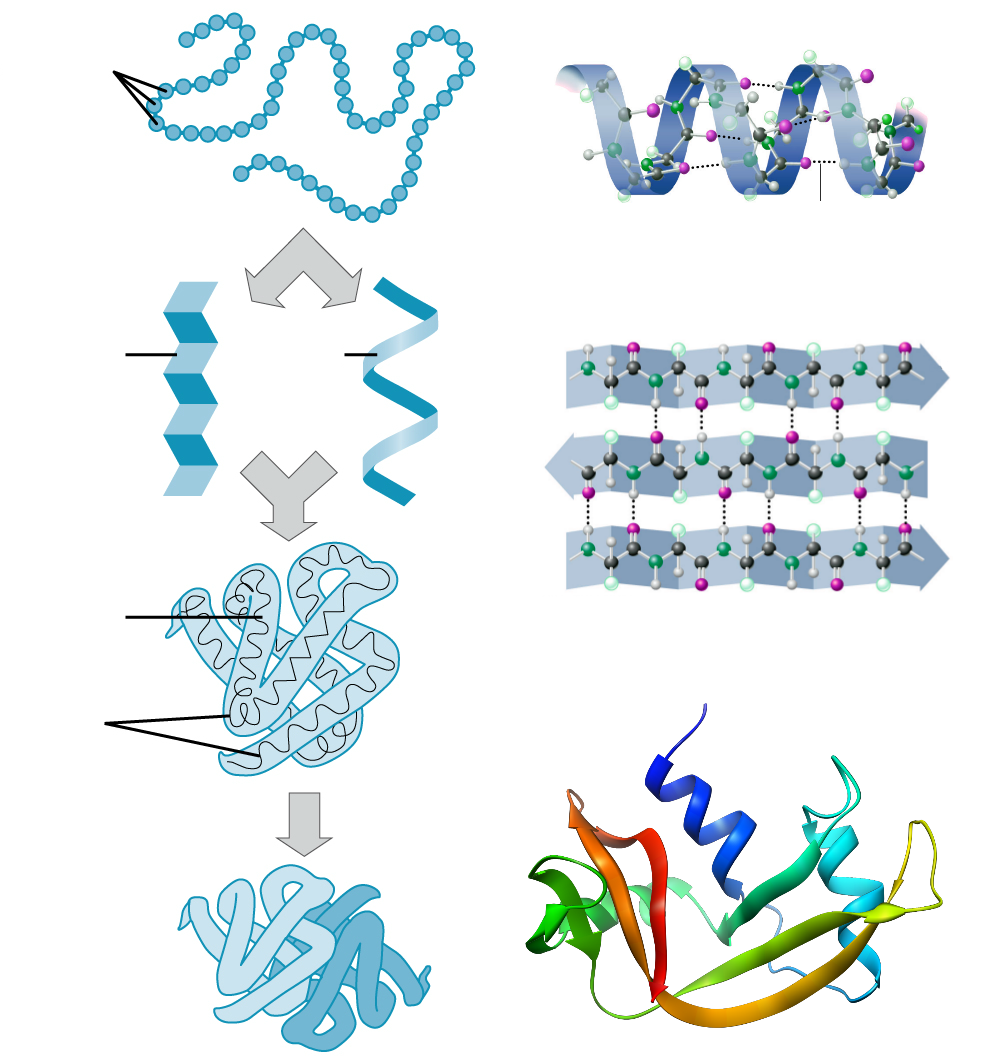
\includegraphics[scale=0.31]{./protein-structure-levels2.png}
}
\caption{
سطوح ساختاری پروتئین.
}
\label{fig:protein}
\end{figure}

\subsection{عملکرد پروتئین}
در فرآیندهای سلولی، پروتئین‌ها نقش اصلی را ایفا می‌کنند. در واقع تمام مولکول‌های دیگر موجود در سلول (به غیر از برخی RNA ها)، عناصری هستند که پروتئین‌ها برای انجام وظایف خود به ‌آن‌ها نیاز دارند و به وسیله‌ی آن‌ها فعالیت خود را انجام می‌دهند. مشخصه اصلی پروتئین‌ها که عملکرد‌های مختلف آن‌ها را نتیجه می‌دهد، توانایی اتصال به مولکول‌ها و پروتئین‌های دیگر است. قسمتی از پروتئین که این توانایی را فراهم می‌آورد، \خمیده{مقر اتصال} نامیده می‌شود که معمولاً به شکل یک حفره در سطح پروتئین واقع می‌گردد. نحوه فعالیت مقر اتصال و خصوصیات آن، توسط زنجیره جانبی اسید‌های آمینه اطراف آن مشخص می‌شود و به قدری خاص منظوره است که حتی یک تغییر کوچک در مولکول چسبنده، مانع از اتصال پروتئین خواهد شد. بنابراین ساختار سوم پروتئین مشخص کننده فعالیت‌ها و عملکرد‌های آن است.

می‌توان فعالیت پروتئین‌ها را به سه دسته کلی تقسیم کرد\جستار{Alberts_2014}:

\paragraph{سیگنال‌دهی و دریافت سیگنال}
به این وسیله پیغام‌هایی در سلول و حتی در سرتاسر بدن پخش می‌شود و واکنش سلول‌ها را به دنبال دارد. به عنوان مثال، انسولین پروتئینی است که نقش سیگنال‌دهی بین سلولی را بر عهده دارد. برخی دیگر از پروتئین‌ها بر روی غشاء سلولی ساکن هستند و نقش دریافت کننده سیگنال و در پی آن، فعال کردن واکنش‌های شیمیایی مناسب در داخل سلول را بر عهده دارند. بعضی پروتئین‌ها به عناصر دیگر می‌چسبند و آن‌ها را علامت‌گذاری می‌کنند. این عناصر علامت‌گذاری شده در فرآیند دیگری مورد استفاده قرار می‌گیرد. به عنوان مثال، پادتن‌ها پروتئین‌هایی هستند که با اتصال به عناصر خارجی، آن‌ها را برای از بین رفتن علامت‌گذاری می‌کنند.

\paragraph{نقش ساختاری}
ناخن، مو، پر و سایر ساختارهای سفت و محکم موجودات از پروتئین‌های ساختاری تشکیل شده‌است. اسکلت سلولی\پانوشت{\متن‌لاتین{cytoskeleton}} نیز از پروتئین‌های ساختاری آکتین\پانوشت{actin} و تبولین\پانوشت{tubulin} ساخته می‌شود.

\paragraph{نقش آنزیمی} 
آنزیم‌ها بزرگترین و مهم‌ترین دسته از پروتئین‌ها هستند. آن‌ها واکنش‌های شیمیایی را تسریع می‌کنند بدون آنکه خود در این واکنش‌ها تغییر یابند. آنزیم‌ها خاص منظوره هستند و معمولاً  هر کدام تنها روی یک یا چند واکنش تأثیرگذار است. حدود ۱۸۰۰۰ واکنش شناسایی شده‌اند که توسط آنزیم‌ها تسریع می‌شوند\جستار{Lang_2011} و برای ۸۷۰۰۰ آنزیم، ساختار سوم مشخص وجود دارد\جستار{Schomburg_2012}. آنزیم‌ها را می‌توان بر اساس عملکرد دسته‌بندی کرد. مهمترین دسته‌بندی آنزیم‌ها بر اساس عدد EC\پانوشت{\متن‌لاتین{Enzyme Commission number}} است. این عدد مشخص می‌کند که هر آنزیم روی چه واکنشی تأثیرگذار است.


\section{پیشبینی عملکرد پروتئین}
 روش‌های آزمایشگاهی برای تشخیص عملکرد پروتئین پر هزینه هستند. بنابراین سعی می‌شود ابتدا با روش‌های محاسباتی، برای هر پروتئین عملکردی پیش‌بینی گردد و سپس در آزمایشگاه درستی این پیش‌بینی آزمون شود. این روش‌های محاسباتی پیش‌بینی، بر اساس تخصیص عملکرد به پروتئین ناشناخته بر مبنای عملکردهای شناخته شده برای پروتئین‌های مشابه، کار می‌کنند. معیارهای مختلفی برای اندازه‌گیری شباهت بین دو پروتئین تعریف شده‌است که از مهمترین آن‌ها می‌توان به روش‌های هم‌ترازی توالی\پانوشت{\متن‌لاتین{sequence alignment}} (مثل \متن‌لاتین{PSI-BLAST}\جستار{Altschul_1997} و \متن‌لاتین{FASTA}\جستار{Pearson_1988}) و هم‌ترازی ساختار\پانوشت{\متن‌لاتین{structure alignment}} (مثل \متن‌لاتین{DALI}\جستار{Holm_1996} و \متن‌لاتین{CE}\جستار{Shindyalov_1998}) اشاره کرد. این روش‌ها بر این مبنا استوارند که پروتئین‌های مشابه از لحاظ ساختاری، به احتمال زیاد از یک جد مشترک\پانوشت{\متن‌لاتین{common ancestor}} تکامل یافته‌اند پس باید عملکرد مشابهی داشته باشند\جستار{Reeck_1987}. بر همین اساس باید گفت در سیر تکامل، ساختار سه‌بعدی پروتئین‌ها کمتر دستخوش تغییر می‌شود\جستار{Illergaard_2009}. پس استفاده از آن برای اندازه‌گیری شباهت، نتایج بهتری بدست خواهد داد. ولی همیشه اینگونه نیست: ممکن است پروتئین‌ها با ساختار مشابه، عملکردهای متفاوت و پروتئین‌های با عملکرد مشابه، ساختار متفاوتی داشته باشند\جستار{Whisstock_2003}. برای در نظر گرفتن این حالت، روش‌های جدید، علاوه بر ساختار، اطلاعات دیگری از پروتئین (نظیر مقر اتصال\پانوشت{\متن‌لاتین{binding site}}\جستار{Binkowski_2003}، تعاملات پروتئینی\جستار{Xenarios_2002} و موتیف‌های اسیدآمینه\پانوشت{amino-acid motifs}\جستار{Yao_2003}) را در تصمیم‌گیری دخیل می‌کنند که می‌توان آن‌ها را به طور کلی به دو دسته تقسیم کرد. روش‌هایی نظیر \متن‌لاتین{ProKnown}\جستار{Pal_2005} و \متن‌لاتین{ProFunc}\جستار{Laskowski_2005} هر منبع اطلاعات را به صورت جداگانه استفاده می‌کنند. به این صورت که در هر منبع، پروتئین‌های مشابه با پروتئین مورد سؤال را مشخص کرده و سپس این اطلاعات را برای رتبه‌بندی پروتئین‌ها بر اساس شباهت استفاده می‌کنند. در روش دوم برای استفاده از اطلاعات مختلف، یک مدل احتمالاتی توام\پانوشت{\متن‌لاتین{joint probabilistic model}} تشکیل می‌شود. دابسن\پانوشت{Dobson} و دویگ \پانوشت{Doig} پروتئین‌ها را به شکل بردارهایی از خصوصیات فیزیکی و شیمیایی نشان دادند و از SVM برای یادگیری روی این بردارها استفاده کردند\جستار{Dobson_2003}. در این حالت می‌توان از هر منبع اطلاعاتی و هر نوع داده‌ای برای گسترش بردار منتسب به هر پروتئین استفاده کرد.

تلاش‌های زیادی برای بهبود مدل دابسن و دویگ هم از نظر سرعت اجرا و هم از نظر دقت، صورت گرفته است. در این بین، راهکارهای مبتنی بر گراف کرنل مورد توجه این پایان‌نامه هستند. گراف کرنل‌های گشت تصادفی (بخش \ارجا{sec:random-walk-kernels})، کوتاهترین مسیر (بخش \ارجا{sec:random-walk-kernels})، گرافلت کرنل (بخش \ارجا{sec:subgraph-kernels}) و خانواده کرنل‌های ویسفلر-لیمن (بخش \ارجا{sec:weisfeiler-lehman-kernels}) همگی در جهت بهبود این مدل استفاده شده‌اند. در ادامه، کاربرد گرافلت کرنل گاوسی در پیش‌بینی عملکرد پروتئین را بررسی می‌کنیم و نشان خواهیم داد که این کرنل توانایی بیشتری برای پیش‌بینی عملکرد پروتئین دارد.

\subsection{شرایط آزمون}
برای آزمون و مقایسه روش‌ها، از زبان برنامه نویسی \متن‌لاتین{C++} جهت پیاده‌سازی کرنل‌ها و محاسبه ماتریس کرنل و از زبان \متن‌لاتین{R} به منظور یادگیری روی ماشین \متن‌لاتین{C-SVM} و تحلیل داده‌ها استفاده کردیم. برای جلوگیری از تأثیر افراز تصادفی داده‌ها بر روی نتایج، آزمایش را در قالب \متن‌لاتین{10-fold cross validation}، ده بار تکرار کردیم. مدت زمان اجرا، در قالب ثانیه و اندازه‌گیری شده بر روی سیستمی با ۴ گیگابایت حافظه و پردازشگر ۲.۶۶ گیگاهرتز اینتل دو هسته‌ای گزارش می‌شود.

\subsection{پایگاه‌های داده}
معمولاً برای بررسی راهکارهای پیش‌بینی عملکرد پروتئین مبتنی بر گراف کرنل، از دو پایگاه داده \متن‌لاتین{ENZYMES} و \متن‌لاتین{DD} استفاده می‌شود. \متن‌لاتین{ENZYMES} پایگاه داده متشکل از ۶۰۰ آنزیم در ۶ دسته است (۱۰۰ پروتئین از ۶ دسته اول عدد \متن‌لاتین{EC}) که از \جستار{Borgwardt_2005} استخراج شده‌است. \متن‌لاتین{DD} پایگاه داده متشکل از ۱۱۷۸ پروتئین در دو دسته است (۶۹۱ پروتئین آنزیمی و ۴۸۷ پروتئین غیرآنزیمی) که توسط دابسن و دویگ گردآوری شده‌است\جستار{Dobson_2003}. پروتئین‌های این پایگاه طوری گردآوری شده‌اند که هیچ زنجیره‌ای از هر پروتئین با هیچ زنجیره دیگری در این پایگاه با z-score بزرگتر از ۳.۵ هم‌تراز نمی‌شود مگر در همان پروتئین. در واقع این پایگاه برای نشان‌دادن ناکارآمدی روش‌های هم‌ترازی توالی ایجاد شده‌است. جدول \ارجا{tab:dataset-statistics} به طور خلاصه جنبه‌های آماری این پایگاه‌ها را نمایش می‌دهد.

\begin{table}[ht]
\centering
\begin{tabular}{| c | c | c | c | c | c |}
    \hline
    نام پایگاه & اندازه & دسته‌ها & $\bar{n}$ & $\bar{m}$ & $\bar{d}$\\[5pt] \hline
    D\&D & 1178 & 2 (691 در مقابل 487) & 263 & 718.5 & 10.03 \\ \hline
    ENZYMES & 600 & 6 (100 تا در هر دسته) & 255 & 691.2 & 9.91 \\ \hline
\end{tabular}
\caption{
    پایگاه‌های داده مورد استفاده و خصوصیات آن‌ها.
 $\bar{n}$: میانگین اندازه گراف‌ها. $\bar{m}$: میانگین تعداد یال‌های هر گراف.  $\bar{d}$: میانگین بیشترین درجه هر گراف.
}
\label{tab:dataset-statistics}
\end{table}

\subsection{تبدیل پروتئین به گراف}
طبیعی است که برای استفاده از یک گراف کرنل روی پروتئین‌ها، ابتدا باید آن‌ها را به صورت گراف مدل کرد. به همین منظور، معمولاً اسید‌های آمینه را به عنوان رئوس گراف در نظر می‌گیرند. بین هر دو رأس یال خواهد بود اگر اسیدهای آمینه متناظر حداکثر به فاصله تعریف شده $d$ از یکدیگر قرار گرفته باشند. به این فاصله، فاصله اتصال\پانوشت{\متن‌لاتین{contact distance}} می‌گوییم. برای اندازه‌گیری این فاصله، باید موقعیت هر اسیدآمینه در فضای سه بعدی را تعیین کرد. اما همانطور که در بخش \ارجا{sec:protein-structure} به آن اشاره شد، هر اسیدآمینه از چند اتم ساخته شده است. اینکه موقعیت اسیدآمینه توسط کدام اتم تعیین شود و فاصله اتصال چقدر باشد، موضوعی چالش برانگیز در تحقیقات بوده است. در بین مقالات مختلف، کربن آلفا 
($C_\alpha$)
، کربن بتا
($C_\beta$)
، ستون اسیدآمینه\پانوشت{backbone} ($BB$)، زنجیره جانبی ($SC$)، تمام اتم‌ها ($ALL$) و ترکیبات مختلف آن‌ها (مثل $C_\alpha+C_\beta$)، برای تعیین موقعیت اسید‌های آمینه استفاده شده‌اند. همچنین فواصل اتصال مختلفی بین ۴ تا ۱۶ آنگسترم در بین مقالات دیده می‌شود\جستار{Filippis_2012}.

از بین تمام حالات ممکن، ما هشت حالت مدل‌سازی پروتئین‌ها در قالب گراف که بیشترین تکرار بین مقالات داشته‌اند را روی دو پایگاه‌داده ENZYME و DD پیاده می‌کنیم. این حالات به ترتیب شامل در نظر گرفتن اتم کربن آلفا با فاصله ۸ آنگسترم، تمام اتم‌ها با فاصله ۵ آنگسترم، اتم کربن بتا با فاصله ۸ آنگسترم، تمام اتم‌ها با فاصله ۴.۵ آنگسترم، اتم کربن آلفا با فاصله ۸.۵ آنگسترم، تمام اتم‌ها با فاصله ۶ آنگسترم، و اتم کربن آلفا با فاصله ۷ و ۶ آنگسترم هستند که در شکل \ارجا{fig:rig-occurance} به ترتیب میزان تکرار در مقالات نمایش داده شده‌اند (بخش ۲.۳.۴ از \جستار{Filippis_2012} را ببینید).

\begin{figure}[ht]
\center{
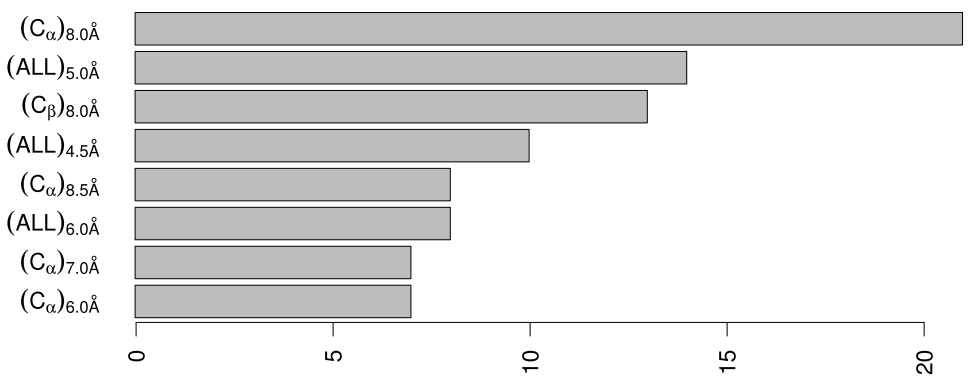
\includegraphics[scale=0.4]{./rig-occurance.png}
}
\caption{پر کاربرد‌ترین اتم‌ها و فواصل برای تبدیل پروتئین به گراف در بین ۲۰۰ مقاله. استخراج شده از \جستار{Filippis_2012}}
\label{fig:rig-occurance}
\end{figure}

\subsection{مقایسه گرافلت کرنل گاوسی و گرافلت کرنل}
در این بخش به مقایسه گرافلت‌کرنل گاوسی (GGK) و گرافلت کرنل (GK) ارائه شده توسط شرواشیتز\جستار{Shervashidze_2009} می‌پردازیم. همانطور که قبلاً ذکر شد، \متن‌لاتین{GK} حاصل ضرب‌داخلی بردار زیرگراف‌های کوچک پروتئین‌هاست. اگرچه نویسنده به این بردار، نام \خمیده{بردار گرافلت} را داده‌است، اما باید توجه داشت که در این کرنل، هر زیرگراف کوچک اعم از القایی یا غیر القایی، همبند یا ناهمبند، گرافلت تلقی می‌شود. به دلیل کُند بودن شمارش تمام زیرگراف‌های همبند یا ناهمبند، تعداد آن‌ها توسط یک تکنیک نمونه‌برداری تخمین زده می‌شود. شکل \ارجا{fig:gk-ggk-accuracy} دقت دسته‌بندی انواع مختلف GK را در مقابل GGK برای دو پایگاه‌داده DD و ENZYMES نمایش می‌دهد. در این شکل، \متن‌لاتین{\خمیده{A}} به معنی شمارش تمام زیرگراف‌های همبند و ناهمبند و \متن‌لاتین{\خمیده{C}} به معنی شمارش زیرگراف‌های فقط همبند است. عددی که بلافاصله بعد از \متن‌لاتین{\خمیده{A}} و \متن‌لاتین{\خمیده{C}} آمده است، اندازه زیرگراف‌های شمارش شده را نشان می‌دهد. اعداد ۲۰۰۰، ۴۰۰۰ و ۸۰۰۰ تعداد نمونه‌ها برای تخمین بردارهای گرافلتی است.

برای ENZYME ، کرنل GGK دارای دقت ۶۴٪ و در مقابل بهترین نتیجه برای GK برابر ۳۸٪ است. همینطور برای DD ، کرنل GGK توانست به دقت ۸۰٪ برسد. این درحالی است که بازهم بهترین نتیجه برای GK ، ۷۷٪ بود. علاوه بر این، GGK سرعت اجرا را فوق‌العاده افزایش داده‌است. همانطور که در جدول \ارجا{tab:ggk-gk-runtime} مشخص است، GGK روی ENZYME حداقل ۱۰ بار سریعتر از پرسرعت‌ترین نوع GK است. برای DD نیز اعداد مشابهی دیده می‌شود: GGK حدود ۱۳ بار سریعتر از سریعترین نوع GK است.

دو کرنل GGK و \متن‌لاتین{GK C5} از نظر نوع گرافلت‌ها کاملاً مشابه هستند. دلیل تفاوت دقت آن‌ها استفاده GGK از تابع کرنل گاوسی برای مقایسه تشابه دو بردار گرافلتی است در حالی که GK تنها به ضرب داخلی دو بردار اکتفا می‌کند.

\begin{figure}[h]
\centering
    \begin{subfigure}[t]{0.5\textwidth}
        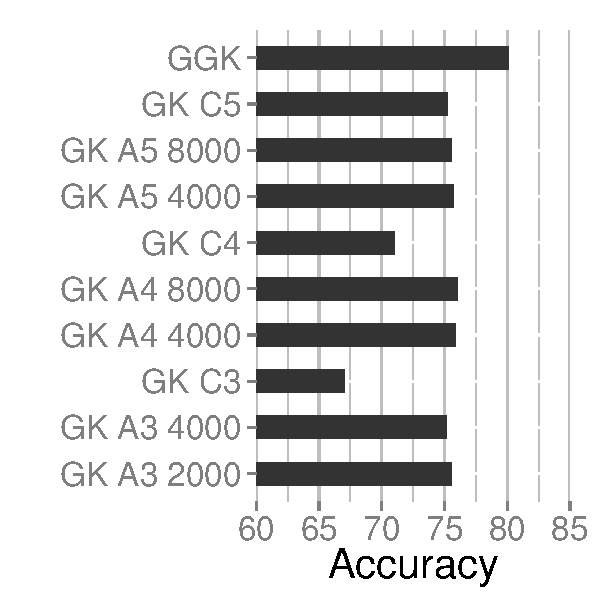
\includegraphics[width=\textwidth]{./dd-ggk-gk.pdf}
        \caption{DD}
    \end{subfigure}%
~
    \begin{subfigure}[t]{0.5\textwidth}
        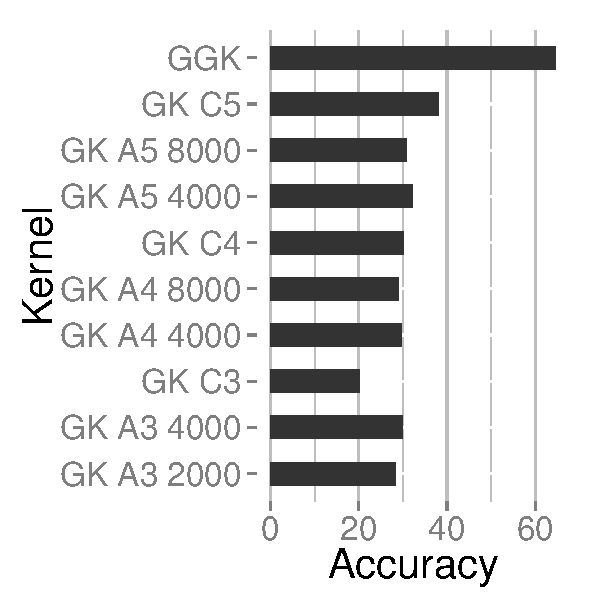
\includegraphics[width=\textwidth]{./enzymes-ggk-gk.pdf}
        \caption{ENZYME}
    \end{subfigure}
\caption{گرافلت کرنل گاوسی (GGK) و انواع گرافلت کرنل (GK). در این شکل، \متن‌لاتین{GK C5}، \متن‌لاتین{GK C4} و \متن‌لاتین{GK C3} گرافلت کرنل‌هایی هستند که به ترتیب تمام گرافلت‌های ۵، ۴ و ۳ رأسی را می‌شمارند. \متن‌لاتین{GK A5}، \متن‌لاتین{GK A4} و \متن‌لاتین{GK A3} گرافلت کرنل‌هایی هستند که به ترتیب تمام گرافلت‌های همبند و ناهمبند ۵، ۴ و ۳ رأسی را می‌شمارند. اعداد ۲۰۰۰، ۴۰۰۰ و ۸۰۰۰ نشان‌دهنده اندازه نمونه انتخاب شده برای تخمین تعداد گرافلت‌هاست.}
\label{fig:gk-ggk-accuracy}
\end{figure}

\begin{table}[th]
\centering
\begin{tabular}{|c|c|c|}
    \hline
کرنل/پایگاه داده & ENZYME & DD \\ \hline\hline
    \lr{GGK} & \lr{0'4"} & \lr{0'8"} \\ \hline\hline
    \lr{GK C5} & \lr{2h 3'8"} & \lr{4h 33'52"} \\ \hline
    \lr{GK A5 8000} & \lr{28'30"} & \lr{1h 26'10"} \\ \hline
    \lr{GK A5 4000} & \lr{21'17"} & \lr{1h 12'15"} \\ \hline\hline
    \lr{GK C4} & \lr{10'24"} & \lr{22'33"} \\ \hline
    \lr{GK A4 8000} & \lr{11'50"} & \lr{24'18"} \\ \hline
    \lr{GK A4 4000} & \lr{6'4"} & \lr{12'33"} \\ \hline\hline
    \lr{GK C3} & \lr{0'48"} & \lr{1'44"} \\ \hline
    \lr{GK A3 4000} & \lr{5'29"} & \lr{11'8"} \\ \hline
    \lr{GK A3 2000} & \lr{2'47"} & \lr{5'44"} \\ \hline
\end{tabular}
\caption{مدت زمان محاسبه ماتریس کرنل برای کرنل GGK و انواع کرنل GK}
\label{tab:ggk-gk-runtime}
\end{table}


\subsection{مقایسه گرافلت کرنل گاوسی و دیگر گراف کرنل‌ها}
در این بخش به مقایسه گرافلت کرنل گاوسی و بهترین گراف کرنل‌های موجود یعنی گراف کرنل گشت تصادفی، گراف کرنل کوتاه‌ترین مسیر، و خانواده گراف کرنل‌های ویسفلر-لیمن (WL) می‌پردازیم.

جداول \ارجا{tab:ggk-vs-others} و \ارجا{tab:ggk-vs-others-runtime} دقت دسته‌بندی و زمان‌اجرای این کرنل‌ها روی پایگاه‌های داده ENZYME و DD را نشان می‌دهند. به منظور سهولت مقایسه، مقادیر \متن‌لاتین{GK C5} را از بخش قبل، به این جداول اضافه می‌کنیم.  برای کرنل‌های ویسفلر-لیمن، پارامتر ارتفاع را برابر ۳ در نظر می‌گیریم. دلیل این انتخاب، تاکید نویسنده به بهینه بودن این ارتفاع (بخش ۴.۲.۲ از \جستار{Shervashidze_2011} را ببینید.) و همچنین صرفه‌جویی در مصرف حافظه است. برای اعداد بزرگتر، مقدار حافظه مورد نیاز این کرنل‌ها به حدی بالا می‌رود که دیگر قادر به محاسبه هیچ کدام از آن‌ها نخواهیم بود.

با توجه به جداول، برای هر دو پایگاه داده ENZYME و DD ، کرنل GGK بهترین عملکرد را داشته است به طوری که به ترتیب، بهترین نتایج روی این پایگاه‌ها را ۵٪ و ۴٪ بهبود داده‌است.

امکان اجرای برخی از کرنل‌ها بر روی پایگاه داده DD وجود نداشت. کرنل ویسفیلر-لیمن یالی، نیاز به حافظه زیادی دارد که بر روی سیستم با ۴ گیگابایت رم قابل اجرا نبود. هرچند امکان اجرای این کرنل بر روی یک سیستم با حافظه بالاتر وجود دارد، اما در صورت استفاده از یک پایگاه داده بزرگتر، بازهم با این مشکل روبرو خواهیم شد و نمی‌توان از این مسئله به سادگی عبور کرد. برای کرنل کوتاه‌ترین مسیر نیز چنین اتفاقی رخ می‌دهد و بعد از اجرا، کرنل به سرعت فضای موجود را اشغال کرده و با کمبود فضا مواجه می‌شود. اجرای دو کرنل گشت تصادفی و ویسفلر-لیمن کوتاه‌ترین مسیر، بیش از یک روز به طول انجامید بنابراین از ادامه کار آن‌ها جلوگیری شد زیرا مقایسه در این حالت معنای خاصی نداشت.


\begin{table}[t]
\centering
\begin{tabular}{|c|c|c|}
    \hline
    کرنل/پایگاه داده & ENZYMES & DD \\ \hline
    \lr{GGK} & \lr{64.68 (±0.67)} & \lr{80.08 (±0.39)} \\ \hline
    \lr{GK C5} & \lr{38.06 (±1.35)} & \lr{75.20 (±0.71)} \\ \hline
    \lr{WL subtree} & \lr{53.06 (±1.26)} & \lr{76.69 (±0.69)} \\ \hline
    \lr{WL edge} & \lr{53.78 (±1.26)} & - \\ \hline
    \lr{WL shortest path} & \lr{59.05 (±1.05)} & - \\ \hline
    \lr{Random Walk} & \lr{21.68 (±0.94)} & - \\ \hline
    \lr{Shortest Path} & \lr{41.68 (±1.79)} & - \\ \hline
\end{tabular}
\caption{دقت دسته بندی ($\pm$ انحراف معیار) 
کرنل‌های مختلف روی پایگاه‌های ENZYME و DD.}
\label{tab:ggk-vs-others}
\end{table}

\begin{table}[t]
\centering
\begin{tabular}{|c|c|c|}
    \hline
    کرنل/پایگاه داده & ENZYMES & DD \\ \hline
    \lr{GGK} & \lr{4"} & \lr{8.54"} \\ \hline
    \lr{GK C5} & \lr{2h 3'8"} & \lr{4h 33'52"}  \\ \hline
    \lr{WL subtree} & \lr{20"} & \lr{2'35"} \\ \hline
    \lr{WL edge} & \lr{11"} & - \\ \hline
    \lr{WL shortest path} & \lr{1'3"} & - \\ \hline
    \lr{Random Walk} & \lr{12'19"} & - \\ \hline
    \lr{Shortest Path} & \lr{5"} & - \\ \hline
\end{tabular}
\caption{
مدت زمان اجرای گراف کرنل‌ها روی دو پایگاه ENZYME و DD. خطوط تیره، کمبود حافظه و یا مدت زمان بیش از یک روز محاسبه را نشان می‌دهند.
}
\label{tab:ggk-vs-others-runtime}
\end{table}

\section{جمع‌بندی}